\documentclass{beeper}

\usepackage{listings}

\title{Git Good}
\subtitle{How to understand Git}
\author{Sumner Evans}
\institute{Mines ACM}
\date{14 February 2023}

\makeatletter
\patchcmd{\beamer@sectionintoc}{\vskip1.5em}{\vskip0.5em}{}{}
\makeatother

\begin{document}

\begin{frame}{A bit about me}
    My name is Sumner, I'm a \textbf{software engineer at Beeper}.
    \begin{itemize}
        \item I graduated from Colorado School of Mines in 2018 with my
            bachelor's in CS and 2019 with a master's in CS.
        \item I am an adjunct professor. Currently I'm teaching CSCI 341. I've
            taught 400, 406, and 564 in the past as well.
        \item I enjoy skiing, volleyball, and soccer.
        \item I'm a 4th degree black belt in ATA taekwondo.
    \end{itemize}
\end{frame}

\begin{frame}{Overview}
    \setbeamertemplate{section in toc}[sections numbered]
    \tableofcontents[hideallsubsections]

    \begin{block}{This talk is interactive!}
        If you have questions at any point, feel free to interrupt me.
    \end{block}
\end{frame}

\section{Why use Git?}

\begin{frame}{Example Scenario 1}

    \begin{enumerate}[<+->]
        \item You start a project called ``my-proj'' and write a ton of code.
        \item You finally get it to (kinda) work.
        \item You decide to make a copy of ``my-proj'' for backup purposes.
        \item You continue development on ``my-proj'' but then screw something
            up really bad.
        \item You decide to revert back to your copy.
        \item Then you realize your copy doesn't have a bug fix that you
            actually wanted.
        \item You then proceed to manually compare the files in the backup to
            those in your new code and figure out what you still want to have.
    \end{enumerate}

    \uncover<8>{This is terrible.}
\end{frame}

\begin{frame}{Example Scenario 2}

    \begin{enumerate}[<+->]
        \item You start working on a project with a partner.
        \item You write a bunch of code.
        \item You email the code in a \texttt{.zip} file, then go home for the
            weekend.
        \item You and your partner had decided to work on two separate tasks
            over the weekend so you make some changes to the code and your
            partner makes some changes to the code.
        \item You come together and start copying files. Then you realize you
            both modified \texttt{main()}.
        \item You then manually determine what changed in both files and
            reconcile them.
    \end{enumerate}

    \uncover<7>{This is awful.}
\end{frame}

\begin{frame}{Version Control Systems}

    Version Control Systems (VCSs) such as Git solve these problems.

    \begin{itemize}[<+->]
        \item VCS keeps track of \textit{revisions}, changes in the code in
            entities called \textit{changesets} or \textit{commits}.
        \item Most VCS allow version merging. That means multiple people can be
            working on the same file and resolve discrepancies later. Git is
            very elegant in handling merge conflicts such as this.
    \end{itemize}
\end{frame}

\begin{frame}{Git is popular}

    Git is a very popular version control system.

    Services such as GitHub and GitLab provide free hosting for Git
    repositories.

    It has become the de-facto industry standard for source control.

\end{frame}

\begin{frame}{Git is a distributed version control system}
    \textbf{Distributed} because you can use it without being connected to a
    central server. You have a full copy of the code on your own computer.

    \textbf{Version control} because it keeps track of changes to files.

    \pause

    \textbf{But how does it keep track of all of the changes?}
\end{frame}

\section{Commits}

\begin{frame}{Commits: what are they?}
    \textbf{Commits} are sets of differences (diffs) in
    files.\footnote[frame]{This is a bit of a lie, more on that later.}
    \pause

    Commits reference their parent(s) and contain information about the changes
    made in the repo since that parent commit.

    \begin{center}
        \only<2>{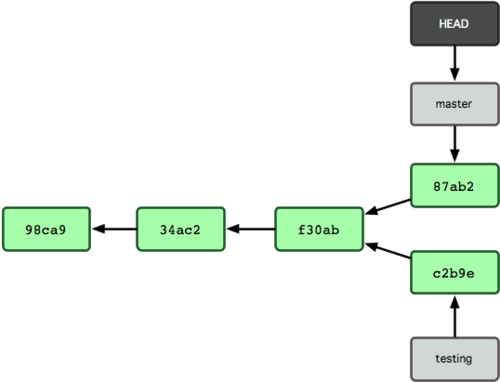
\includegraphics[height=55mm]{graphics/branching5}}
    \end{center}
\end{frame}

\begin{frame}{Commits: they form a DAG, and are stored on the ``heap''}

    Commits form a Directed Acyclic Graph (DAG). There are no loops in the
    graph, and every commit points to its parent(s).

    Every single commit is stored in the \texttt{.git} directory of your
    repository\footnote[frame]{Technically another lie.} which can be thought of
    like a ``heap'' for commits. The parents of a commit are also stored in this
    ``heap''.

    We will return to this fact when we talk about \textit{branches}.

\end{frame}

\begin{frame}{Commits: creating}
    You can create a commit by running \texttt{git commit}. This will create a
    commit based on the checked-out commit with the changes that you have
    ``staged''.
    \pause

    \begin{itemize}[<+->]
        \item You can stage changes by running \texttt{git add} and passing a
            list of files.
        \item You can stage all changes by running \texttt{git add -A}.
        \item \textbf{Pro tip}: If you want to add specific parts of files, use
            \texttt{git add -p}.
    \end{itemize}

    \pause[\thebeamerpauses]
    If you want to remove from the stage, you can run \texttt{git reset}
    (optionally passing a list of files to unstage).
\end{frame}

\begin{frame}[fragile]{Commits: what will be committed?}
    If you ever want to know what will be included in your commit, you can run
    \texttt{git status} to show the list of files staged for commit.
    \pause

    {
        \tiny
        \begin{minted}{text}
        > git status
        On branch master
        Your branch is up to date with 'origin/master'.

        Changes to be committed:
          (use "git restore --staged <file>..." to unstage)
                modified:   git.tex

        Changes not staged for commit:
          (use "git add <file>..." to update what will be committed)
          (use "git restore <file>..." to discard changes in working directory)
                modified:   git.pdf
                modified:   git.tex
        \end{minted}
    }

    \pause
    The \texttt{git.tex} file has only some lines staged for commit.
\end{frame}

\begin{frame}[fragile]{Commits: what will be committed, but with more detail?}
    To see the details of the changes that are staged (that is, will be
    committed), you can run \texttt{git diff --cached}.

    If you want to see the details of the changes that are \textit{not} staged,
    you can run \texttt{git diff}.

    \texttt{git diff} optionally accepts a list of files to diff.
    \pause

    {
        \tiny
        \begin{minted}{text}
            diff --git a/git.tex b/git.tex
            index 2c01a7b..91148d1 100644
            --- a/git.tex
            +++ b/git.tex
            @@ -33,9 +33,7 @@

             \section{Why use Git?}

            -\begin{frame}{Why use Git? I}
            -
            -    Example Scenario:
            +\begin{frame}{Example Scenario 1}

                 \begin{enumerate}[<+->]
                     \item You start a project called ``my-proj'' and write a ton of code.
        \end{minted}
    }
\end{frame}

\begin{frame}{Commits: summary}
    Use \texttt{git add} and \texttt{git reset} (or variants) to stage/unstage
    changes for your.
    \pause

    Use \texttt{git commit} to create a commit from the currently staged changes
    (which you can see by running \texttt{git diff --cached}).
\end{frame}

\section{Branches}

\begin{frame}{Branches: what are they?\footnote[frame]{Info in the rest of the
    \textit{Branches} section is mainly from
    \url{https://git-scm.com/book/en/v2/Git-Branching-Branches-in-a-Nutshell}}}

    Remember how we said that the \texttt{.git} directory is like a ``heap'' for
    commits?

    \textbf{Branches are pointers to a specific commit in that heap.} You can
    then follow that commit's parent pointers to reconstruct the graph.
\end{frame}

\begin{frame}{Branches: pointers}


    \begin{center}
        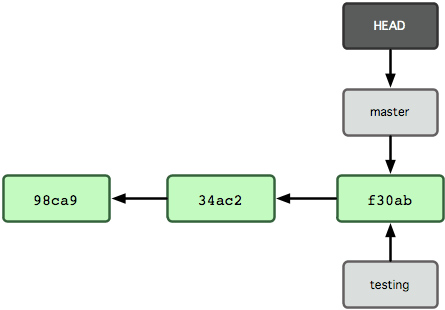
\includegraphics[height=50mm]{graphics/branching1}
    \end{center}
\end{frame}

\begin{frame}{Branches: creating them}
    Branches can be created using the \texttt{git branch <branch name>} command.
    \textbf{This will not change your \texttt{HEAD} pointer.}

    \begin{center}
        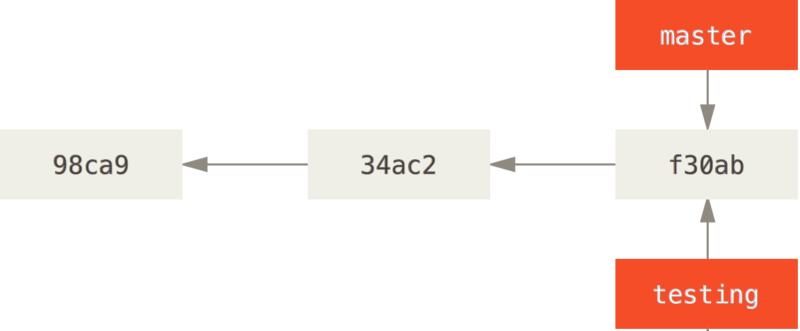
\includegraphics[height=35mm]{graphics/branching-creating}
    \end{center}

    If you want to create a branch and also change the \texttt{HEAD} pointer to
    the newly created branch, you can use:\\
    \texttt{git checkout -b <branch name>}.
    \pause

    You can use \texttt{git branch [-a]} to list (all) branches.
\end{frame}

\begin{frame}{Branches: moving \texttt{HEAD} around}
    \texttt{HEAD} is a special pointer to the current repository state.
    Checking out a commit/branch will update the files in your working
    directory.

    You can move the \texttt{HEAD} pointer to a different commit using\\
    \texttt{git checkout <commit hash or branch name>}.

    \only<1>{\begin{center}
        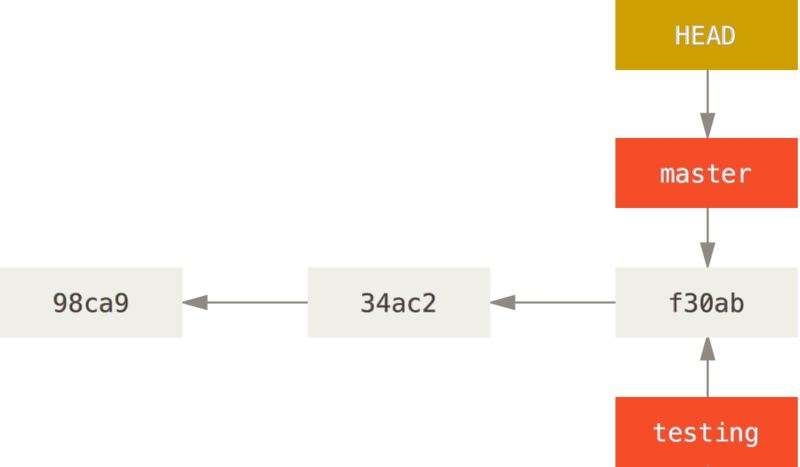
\includegraphics[height=45mm]{graphics/branching-moving-1}
    \end{center}}
    \only<2>{\begin{center}
        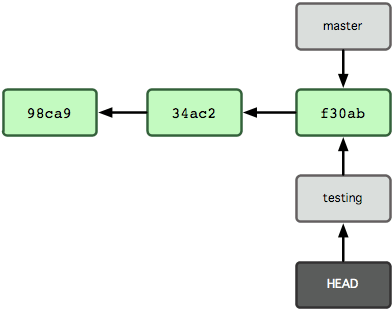
\includegraphics[height=45mm]{graphics/branching2}
    \end{center}}

\end{frame}

\begin{frame}{Branches: \texttt{checkout} gotchas and pro-tips}
    \begin{itemize}
        \item If you checkout a commit hash, you will be in a \texttt{detached
            HEAD} state because your \texttt{HEAD} pointer is not pointing to a
            branch.
            \pause

        \item If you have uncommitted changes, switching branches \textit{might}
            fail.
            \pause

            You can use \texttt{git stash} to save the changes in your working
            directory, then \texttt{checkout} the other branch, and then
            \texttt{git stash pop} to restore the changes.

            Alternatively, you can just create a WIP commit and then switch to
            the other branch.
    \end{itemize}
    \pause

    \textbf{Pro tip}: You can use \texttt{-} to refer to the previously checked
    out object.
\end{frame}

\begin{frame}{Branches: making commits}
    If you commit something while \texttt{HEAD} is pointed to a branch, both
    \texttt{HEAD} and your branch will move to the new commit.

    \only<1>{\begin{center}
        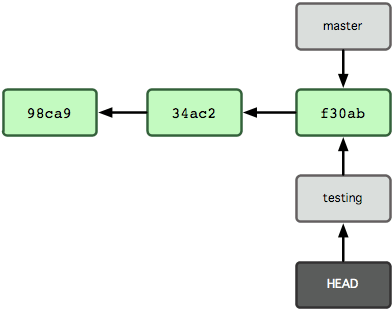
\includegraphics[height=45mm]{graphics/branching2}
    \end{center}}
    \only<2>{\begin{center}
        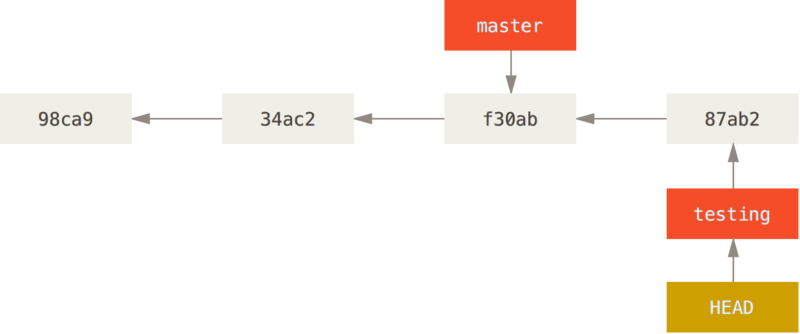
\includegraphics[height=45mm]{graphics/branching3}
    \end{center}}
\end{frame}

\begin{frame}{Branches: using multiple branches}
    Of course, you can always switch back to \texttt{master} using \texttt{git
    checkout master}.

    \begin{center}
        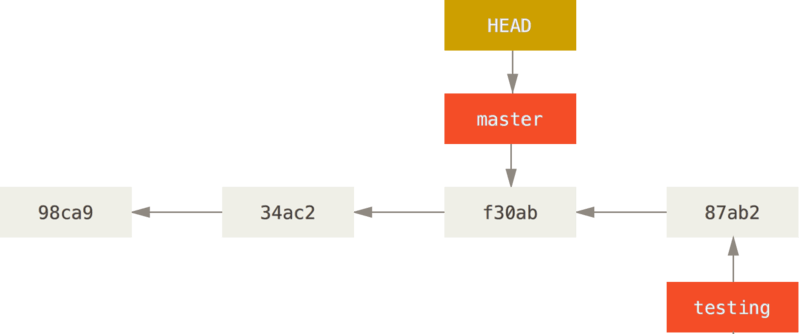
\includegraphics[width=110mm]{graphics/branching4}
    \end{center}
\end{frame}

\begin{frame}{Branches: divergence}
    If you make a commit on the master branch, the \texttt{master} pointer moves
    to that new commit creating \textbf{divergent} branch histories.

    \begin{center}
        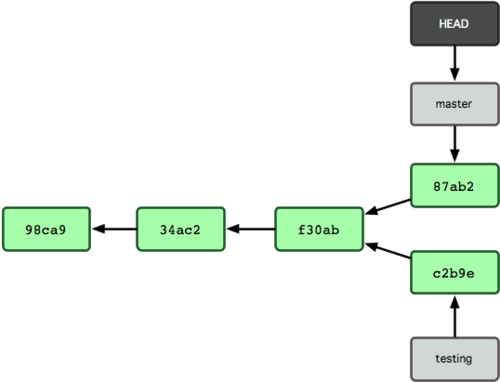
\includegraphics[width=110mm]{graphics/branching5}
    \end{center}
\end{frame}

\begin{frame}[fragile]{Branches: where am I?}
    Often, you want to get a summary of where you are in the repository. That's
    where \texttt{git log} comes in.

    {
        \tiny
        \begin{minted}{text}
            > git log
            commit b08107c144003ba42495995d59234595d2d875b4 (HEAD -> master, origin/master, origin/HEAD)
            Author: Sumner Evans <me@sumnerevans.com>
            Date:   Mon Feb 13 14:35:57 2023 -0700

                fix some things

                Signed-off-by: Sumner Evans <me@sumnerevans.com>

            commit 6c1f8b53ac774dc6b0376810b4745951bd572519
            Merge: 47bc626 67f0f4d
            Author: Ethan Richards <42894274+ezrichards@users.noreply.github.com>
            Date:   Mon Feb 13 14:06:08 2023 -0700

                Merge branch 'master' of github.com:ColoradoSchoolOfMines/mineshspc.com

            ...
        \end{minted}
    }
    \pause
    This is mostly useless. Let's make it better.
\end{frame}

\begin{frame}[fragile]{\texttt{git log}: but actually good}
    For \texttt{git log} to be useful, you want it to show \textit{all}
    branches, show a graph, and get rid of most of the details.

    {
        \tiny
        \begin{minted}{text}
            > git log --all --graph --decorate --oneline
            * b08107c (HEAD -> master, origin/master, origin/HEAD) fix some things
            *   6c1f8b5 Merge branch 'master' of github.com:ColoradoSchoolOfMines/mineshspc.com
            |\
            | * 67f0f4d fix background color bug
            * | 47bc626 Fix accordion
            |/
            * 186b52a Archive overhaul
            * 385666b Fix accordion arrows
            * 3d0f64a Archive preliminary updates
            * aaae02b Update FAQ and archive pages
            *   b2a64f7 Merge branch 'master' of github.com:ColoradoSchoolOfMines/mineshspc.com
            |\
            | * 1450745 make footer reveal
            * | f7ddfa2 Fix alt text
            |/
            * 0f89721 created student confirm registration page
            * 7b15e86 editing teams: ensure that you can't change from in-person to remote or vice versa
            * e15bda6 save team below member list
            * 853dcd1 add ability to add team members
            \end{minted}
    }
\end{frame}

\begin{frame}{Branches: summary}
    \begin{itemize}
        \item Branches are \textbf{pointers} to commits.
        \item Use \texttt{git checkout} to move between branches.
        \item Use \texttt{git log} to see where you are.
    \end{itemize}
\end{frame}

\section{Merging}

\begin{frame}{Merging: resolving divergent histories\footnote[frame]{Info in the rest of the
    \textit{Merging} section is mainly from
    \url{https://git-scm.com/book/en/v2/Git-Branching-Basic-Branching-and-Merging}}}

    If you want to merge the changes from branch \texttt{A} into another branch
    \texttt{B}, you need to:

    \begin{enumerate}
        \item Switch to branch \texttt{B} (\texttt{git checkout B})
        \item Run \texttt{git merge A}.
    \end{enumerate}

    This will do one of two things: fast-forward or create a merge commit.
\end{frame}

\begin{frame}{Merging: fast-forwarding}

    If the branch you are merging is directly ahead of the branch you are
    merging into, Git will just move the pointer in a \textbf{fast-forward
    merge}.

    \begin{center}
        \only<1>{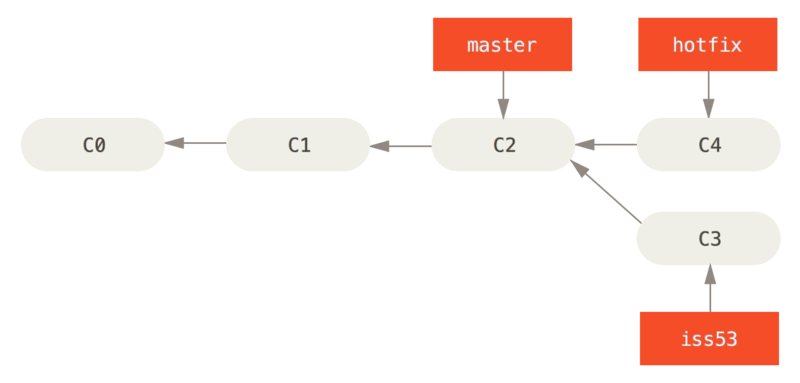
\includegraphics[width=90mm]{graphics/merging-1}}
        \only<2>{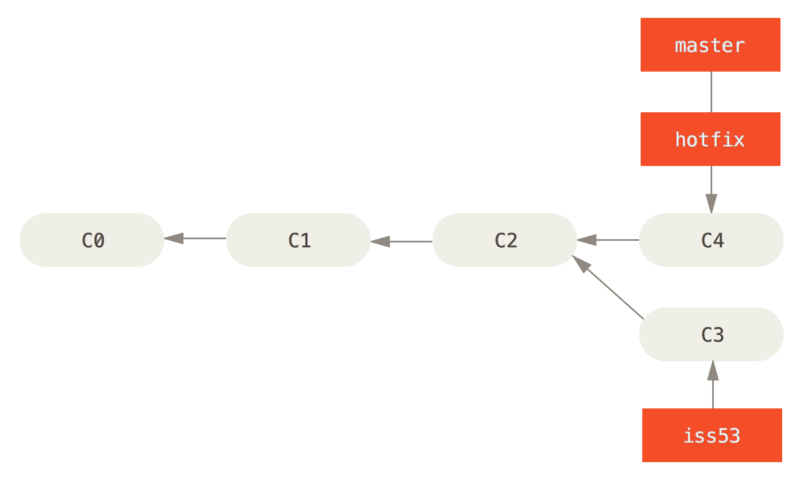
\includegraphics[width=90mm]{graphics/merging-2}}
    \end{center}
\end{frame}

\begin{frame}{Merging: creating a merge commit}
    If the branch you are merging has diverged from the one you are merging
    into, Git will create a merge commit through a \textbf{three-way merge}.

    \begin{center}
        \only<1>{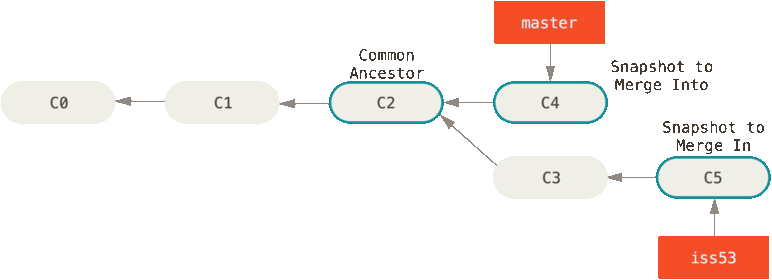
\includegraphics[height=30mm]{graphics/merging-3way-1}}
        \only<2>{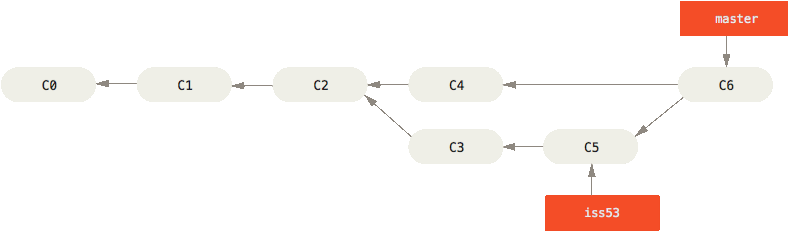
\includegraphics[height=30mm]{graphics/merging-3way-2}}
    \end{center}
\end{frame}

\begin{frame}[fragile]{Merging: resolving conflicts}
    Occasionally, this process doesn't go smoothly. If you changed the same part
    of the same file differently in the two branches you're merging, Git won't
    be able to merge them cleanly.

    {
        \tiny
        \begin{minted}{text}
            > git merge iss53
            Auto-merging index.html
            CONFLICT (content): Merge conflict in index.html
            Automatic merge failed; fix conflicts and then commit the result.
        \end{minted}
    }
    \pause
    You can always use \texttt{git status} to see what has been automatically
    merged and what files have conflicts.
    {
        \tiny
        \begin{minted}{text}
            > git status
            On branch master
            You have unmerged paths.
              (fix conflicts and run "git commit")

            Unmerged paths:
              (use "git add <file>..." to mark resolution)

                both modified:      index.html

            no changes added to commit (use "git add" and/or "git commit -a")
        \end{minted}
    }
\end{frame}

\begin{frame}[fragile]{Merging: editing files to resolve merge conflicts}
    You can use a merge tool to resolve conflicts, however I find that it's
    easier to just manually resolve the conflicts.

    Visual Studio Code has a good UI for this. The process you should follow is
    as follows:

    \begin{enumerate}
        \item Open a file with the conflict.
        \item Find one of the conflict-resolution markers.
        \item Make edits to resolve the conflict.
        \item Run \texttt{git add} on the file.
        \item Repeat steps 1-4 until all conflicts are resolved.
        \item Run \texttt{git commit} to commit the merge.
    \end{enumerate}

\end{frame}

\begin{frame}[fragile]{Merging: understanding conflict-resolution markers}
    In order to find the conflict-resolution markers, search for
    \texttt{<<<<<<<}. Each conflict-resolution block should look something like
    this:
    {
        \tiny
        \begin{minted}{text}
            <<<<<<< HEAD:index.html
            <div id="footer">contact : email.support@github.com</div>
            =======
            <div id="footer">
             please contact us at support@github.com
            </div>
            >>>>>>> iss53:index.html
        \end{minted}
    }

    The first part (between \texttt{<<<<<<<} and \texttt{=======}) is what the
    branch you are merging \textit{into} has. The second part (between
    \texttt{=======} and \texttt{>>>>>>>}) is what the branch you are merging
    \textit{from} has.
    \pause

    Sometimes, you just one one side of the conflict, other times you need to be
    more nuanced in your merge.
\end{frame}

\begin{frame}{Merging: summary}
    \begin{itemize}
        \item Merging allows you to pull changes from one branch into another
            branch.
        \item Use \texttt{git merge A} to merge branch \texttt{A} into the
            current branch.
        \item Git will do a fast-forward merge if possible, otherwise it will
            create a merge commit.
        \item You might have to resolve merge conflicts.
    \end{itemize}
\end{frame}

\section{Rebasing}

\begin{frame}[fragile]{Rebasing: maintaining linear histories}
    Most merge commits are useless. They clutter the history, and normally don't
    add anything of value to the understanding of how the codebase evolved.

    {
        \tiny
        \begin{minted}{text}
            * b08107c (HEAD -> master, origin/master, origin/HEAD) fix some things
            *   6c1f8b5 Merge branch 'master' of github.com:ColoradoSchoolOfMines/mineshspc.com
            |\
            | * 67f0f4d fix background color bug
            * | 47bc626 Fix accordion
            |/
            * 186b52a Archive overhaul
            * 385666b Fix accordion arrows
        \end{minted}
    }
    \pause

    Ideally the above history would be linear:

    {
        \tiny
        \begin{minted}{text}
            * b08107c (HEAD -> master, origin/master, origin/HEAD) fix some things
            * 47bc626 Fix accordion
            * 67f0f4d fix background color bug
            * 186b52a Archive overhaul
            * 385666b Fix accordion arrows
        \end{minted}
    }

\end{frame}

\begin{frame}{Rebasing: what it does}
    Rebasing allows you to take the commits from one branch and reapply them on
    top of another branch.

    \begin{center}
        \only<1>{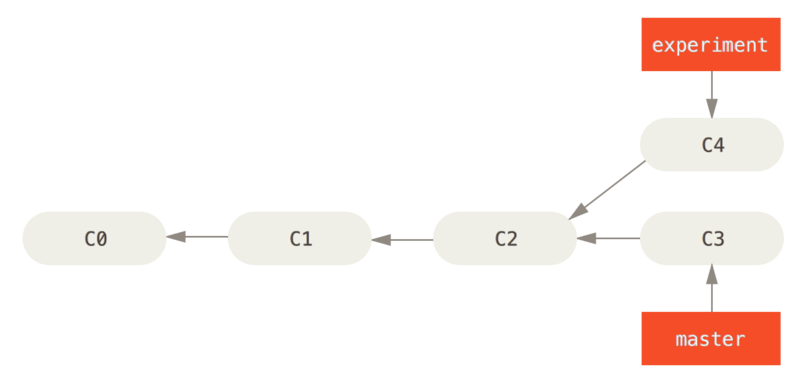
\includegraphics[height=40mm]{graphics/basic-rebase-1}}
        \only<2>{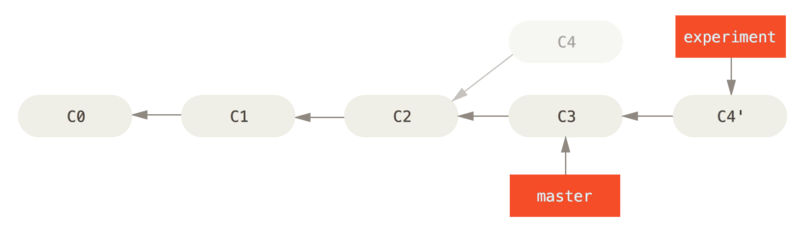
\includegraphics[height=30mm]{graphics/basic-rebase-3}}
    \end{center}
\end{frame}

\section{Remotes}

\begin{frame}{Remotes: what are they?}
    A remote is 
\end{frame}

\section{Advanced Tips}

\begin{frame}{Advanced Topics}
    Gitignore

    Aliases
\end{frame}

\begin{frame}
    \frametitle{How to use Git with a remote}

    \begin{itemize}
        \item Add Remote (\texttt{git remote add [name] [url]}): Adds a
            \textit{remote}, a version of the repository hosted externally from
            your local machine. Most likely on something like Github or an
            company's internal network.
        \item Push (\texttt{git push -u origin master}): Pushes all changes on
            the given branch to the remote.
        \item Clone (\texttt{git clone}): Copies the entire repository to the
            location.
        \item Fetch (\texttt{git fetch}): Retrieves changes from the remote.
        \item Merge (\texttt{git merge}): Merges a branch into another branch.
            (More on branches later, but in this case, we are merging the
            \texttt{origin/master} into our local \texttt{master} branch.)
        \item Pull (\texttt{git pull}): Retrieves any new changes from the
            remote and merges them with your local changes.
    \end{itemize}
\end{frame}

\begin{frame}
    \frametitle{Undoing Things}

    \begin{itemize}
        \item Undo the last $n$ commits (given that you haven't pushed them yet)
            \texttt{git reset --hard HEAD\textasciitilde n}
        \item Undo the $n^{th}$ to last commit by creating a new commit that
            reverts all of the changes \texttt{git revert HEAD\textasciitilde n}
        \item Somebody's done it before. Just Google it.
    \end{itemize}
\end{frame}

\begin{frame}
    \frametitle{The Random Stuff: Stashing}

    When you have changes in your working directory, merges and switching branches (sometimes)
    doesn't work. You have two main options here:

    \begin{enumerate}
        \item Commit your changes. If you can do this, you should.
        \item Occasionally you just don't want to commit. In this case, you will want to
            \textit{stash} your changes using\\ \texttt{git stash [save [stash\_name]]}.
        \item To un-stash, use \texttt{git stash pop}. You may have to resolve merge conflicts.
    \end{enumerate}
\end{frame}

\begin{frame}
    \frametitle{The Random Stuff: Submodules}

    \textbf{What is a submodule?} It is literally a repository inside of another repository.\\

    \textbf{Why is this useful?} If you have a custom library shared between many projects, you can
    place that library in a standalone Git repository. Then you can add it as a submodule to your
    products via \texttt{git submodule add [clone\_url]}.

    The submodule is its own repository so it can be contributed to independently, but it can also
    be modified and contributed to as a submodule.
\end{frame}

\begin{frame}
    \frametitle{The Random Stuff: Aliases}

    As one would expect from something designed and built by Linus Torvalds, Git supports the
    concept of \textit{aliasing} one git command to another name.\\

    For example, you might want to alias \texttt{checkout} to \texttt{co}. This particular alias can
    be achieved using \\ \texttt{git config --global alias.co checkout}.\\

    Now you can invoke \texttt{git checkout} using \texttt{git co}.\\

    Another option is using your shell's alias functionality. This is often more powerful, but that
    isn't part of this talk.
\end{frame}

\begin{frame}
    \frametitle{The Random Stuff: Resources/Tips}

    I obviously was unable to tell you about everything you can do with Git. I've really only
    scratched the surface.

    \begin{itemize}
        \item \texttt{man git *}: The man pages on Git are good. Use them as your first line of
            defense.
        \item \href{https://git-scm.com/book/en/v2}{git-scm.com/book/en/v2}: A
            huge resource about how to do everything Git.
        \item \href{https://gitignore.io}{gitignore.io}: Generates a
            \texttt{.gitignore} file for a given project type, OS, and IDE.
        \item \texttt{git reset --hard HEAD}: Undoes all changes since the last commit.
        \item \texttt{git diff HEAD:file1 file2}: Shows the difference between \texttt{file1} and
            \texttt{file2}.
    \end{itemize}
\end{frame}

\begin{frame}
    \frametitle{Where to Go from Here?}
    \begin{itemize}[<+->]
        \item If you haven't ever used Git, start by using it locally and with Github.
        \item If you know the basics, start exploring branches. Learn about them and find a flow
            which works best for you.
        \item If you know most things about Git, just keep using it. Try and start remembering how
            to do certain things that you find yourself often Googleing for. 
    \end{itemize}
    Become the person everyone asks for Git advice. It's used in the industry, so many companies
    will want to see knowledge of this tool.
\end{frame}

\end{document}
